\section{Fallstudie: Fair Projects}
\label{fallstudie-fair-projects}

Als Beispielanwendung für die Erstellung einer MEAN Anwendung kommt das Problem der Verteilung von Projekten zum Einsatz.
So sind Projektarbeiten im Studienumfeld oft anzutreffen und die zu erarbeitenden Themen sind dabei für die Teilnehmer oftmals vordefiniert.
Jetzt stellt sich das Problem, welcher Teilnehmer, welches Projekt zugeteilt bekommen.
Die Verteilung ist dabei oft recht langwierig.
Um dieses Problem zu lösen ist das Windhundverfahren sehr beliebt. Dort erhält der der zuerst kommt, den Zuschlag erhält.
Das führt meist dazu, dass dies der mit dem am stärksten ausgeprägten Stimmorgan ist. 

Unsere Idee, um dieses Problem fair zu lösen, ist die Verteilung mittels Priorisierung.
Dazu soll eine Webanwendung entwickelt werden, auf die alle Teilnehmer Zugriff haben. 
Dort soll jeder Teilnehmer seine Lieblingsprojekte je nach Wunsch individuell priorisieren können.
Der Ersteller der Projekte soll dabei immer einen Überblick haben, welche Projekte unterbelegt sind und wie die einzelnen Prioritäten der Teilnehmer verteilt sind.
Dadurch soll die aufgewendete Zeit verringert werden und eine möglichst faire Wahl für alle Teilnehmer gewährleistet werden.

Der grundlegende Ablauf dabei sieht folgendermaßen aus:
\begin{itemize}
	\item Die Professoren erstellen für das jeweilige Fach mehrere Projekte mit vollständiger Beschreibung
	\item Die Studenten können anschließend ihre Prioritäten für jedes der Projekte vergeben
	\item Der Professor kann die Projekte anschließend, anhand der Übersichtstabelle mit allen Prioritäten, verteilen
\end{itemize}

Einen ersten Grobentwurf für die Webanwendung ist dabei unter Abbildung \ref{f:fallstudie:firstdraft} zu finden. Dargestellt sind die einzelnen Oberflächen und die Übergänge dazwischen. Benutzer können sich im Fenster oben links einloggen und erhalten danach eine Liste aller Fächer für die eine Umfrage existiert. Diese Fächer können dort auch wieder gelöscht werden. In der ersten Iteration dieser Anwendung wird noch nicht zwischen Personen unterschieden, da es nur als technischer Durchstich dienen soll. Das heißt, dass Person A in der Rolle Student könnte auch wieder Umfragen löschen, die von Person B in der Rolle als Professor erstellt wurden. Ein entsprechendes Rollenkonzept würde in einer der nächsten Iterationen kommen.
Ein Student könnte, wie im Fenster unten links zu sehen ist, an einer Umfrage teilnehmen und seine Prioritäten für die Fächer verteilen.

\begin{figure}[t]
	\centering
	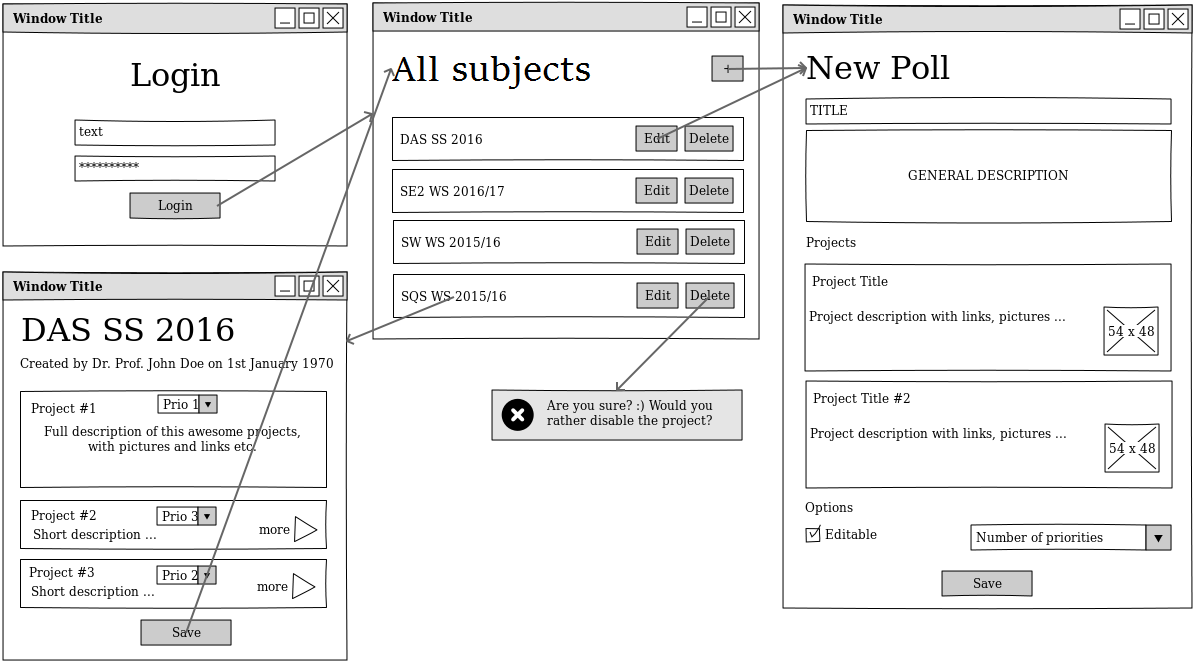
\includegraphics[width=0.7\linewidth]{figures/fairprojectsFirstDraft.png}
	\caption{Erster Entwurf von FairProjects}
	\label{f:fallstudie:firstdraft}
\end{figure}